\documentclass[journal,12pt,twocolumn]{IEEEtran}
\usepackage{setspace}
\usepackage{gensymb}
\usepackage{caption}
%\usepackage{multirow}
%\usepackage{multicolumn}
%\usepackage{subcaption}
%\doublespacing
\singlespacing
\usepackage{csvsimple}
\usepackage{amsmath}
\usepackage{multicol}
%\usepackage{enumerate}
\usepackage{amssymb}
%\usepackage{graphicx}
\usepackage{newfloat}
%\usepackage{syntax}
\usepackage{listings}
\usepackage{iithtlc}
\usepackage{color}
\usepackage{tikz}
\usetikzlibrary{shapes,arrows}



%\usepackage{graphicx}
%\usepackage{amssymb}
%\usepackage{relsize}
%\usepackage[cmex10]{amsmath}
%\usepackage{mathtools}
%\usepackage{amsthm}
%\interdisplaylinepenalty=2500
%\savesymbol{iint}
%\usepackage{txfonts}
%\restoresymbol{TXF}{iint}
%\usepackage{wasysym}
\usepackage{amsthm}
\usepackage{mathrsfs}
\usepackage{txfonts}
\usepackage{stfloats}
\usepackage{cite}
\usepackage{cases}
\usepackage{mathtools}
\usepackage{caption}
\usepackage{enumerate}	
\usepackage{enumitem}
\usepackage{amsmath}
%\usepackage{xtab}
\usepackage{longtable}
\usepackage{multirow}
%\usepackage{algorithm}
%\usepackage{algpseudocode}
\usepackage{enumitem}
\usepackage{mathtools}
\usepackage{hyperref}
%\usepackage[framemethod=tikz]{mdframed}
\usepackage{listings}
    %\usepackage[latin1]{inputenc}                                 %%
    \usepackage{color}                                            %%
    \usepackage{array}                                            %%
    \usepackage{longtable}                                        %%
    \usepackage{calc}                                             %%
    \usepackage{multirow}                                         %%
    \usepackage{hhline}                                           %%
    \usepackage{ifthen}                                           %%
  %optionally (for landscape tables embedded in another document): %%
    \usepackage{lscape}     


\usepackage{url}
\def\UrlBreaks{\do\/\do-}


%\usepackage{stmaryrd}


%\usepackage{wasysym}
%\newcounter{MYtempeqncnt}
\DeclareMathOperator*{\Res}{Res}
%\renewcommand{\baselinestretch}{2}
\renewcommand\thesection{\arabic{section}}
\renewcommand\thesubsection{\thesection.\arabic{subsection}}
\renewcommand\thesubsubsection{\thesubsection.\arabic{subsubsection}}

\renewcommand\thesectiondis{\arabic{section}}
\renewcommand\thesubsectiondis{\thesectiondis.\arabic{subsection}}
\renewcommand\thesubsubsectiondis{\thesubsectiondis.\arabic{subsubsection}}

% correct bad hyphenation here
\hyphenation{op-tical net-works semi-conduc-tor}

%\lstset{
%language=C,
%frame=single, 
%breaklines=true
%}

%\lstset{
	%%basicstyle=\small\ttfamily\bfseries,
	%%numberstyle=\small\ttfamily,
	%language=Octave,
	%backgroundcolor=\color{white},
	%%frame=single,
	%%keywordstyle=\bfseries,
	%%breaklines=true,
	%%showstringspaces=false,
	%%xleftmargin=-10mm,
	%%aboveskip=-1mm,
	%%belowskip=0mm
%}

%\surroundwithmdframed[width=\columnwidth]{lstlisting}
\def\inputGnumericTable{}                                 %%
\lstset{
%language=C,
frame=single, 
breaklines=true,
columns=fullflexible
}
 

\begin{document}
%
\tikzstyle{block} = [rectangle, draw,
    text width=3em, text centered, minimum height=3em]
\tikzstyle{sum} = [draw, circle, node distance=3cm]
\tikzstyle{input} = [coordinate]
\tikzstyle{output} = [coordinate]
\tikzstyle{pinstyle} = [pin edge={to-,thin,black}]

\theoremstyle{definition}
\newtheorem{theorem}{Theorem}[section]
\newtheorem{problem}{Problem}
\newtheorem{proposition}{Proposition}[section]
\newtheorem{lemma}{Lemma}[section]
\newtheorem{corollary}[theorem]{Corollary}
\newtheorem{example}{Example}[section]
\newtheorem{definition}{Definition}[section]
%\newtheorem{algorithm}{Algorithm}[section]
%\newtheorem{cor}{Corollary}
\newcommand{\BEQA}{\begin{eqnarray}}
\newcommand{\EEQA}{\end{eqnarray}}
\newcommand{\define}{\stackrel{\triangle}{=}}

\bibliographystyle{IEEEtran}
%\bibliographystyle{ieeetr}

\providecommand{\nCr}[2]{\,^{#1}C_{#2}} % nCr
\providecommand{\nPr}[2]{\,^{#1}P_{#2}} % nPr
\providecommand{\mbf}{\mathbf}
\providecommand{\pr}[1]{\ensuremath{\Pr\left(#1\right)}}
\providecommand{\qfunc}[1]{\ensuremath{Q\left(#1\right)}}
\providecommand{\sbrak}[1]{\ensuremath{{}\left[#1\right]}}
\providecommand{\lsbrak}[1]{\ensuremath{{}\left[#1\right.}}
\providecommand{\rsbrak}[1]{\ensuremath{{}\left.#1\right]}}
\providecommand{\brak}[1]{\ensuremath{\left(#1\right)}}
\providecommand{\lbrak}[1]{\ensuremath{\left(#1\right.}}
\providecommand{\rbrak}[1]{\ensuremath{\left.#1\right)}}
\providecommand{\cbrak}[1]{\ensuremath{\left\{#1\right\}}}
\providecommand{\lcbrak}[1]{\ensuremath{\left\{#1\right.}}
\providecommand{\rcbrak}[1]{\ensuremath{\left.#1\right\}}}
\theoremstyle{remark}
\newtheorem{rem}{Remark}
\newcommand{\sgn}{\mathop{\mathrm{sgn}}}
\providecommand{\abs}[1]{\left\vert#1\right\vert}
\providecommand{\res}[1]{\Res\displaylimits_{#1}} 
\providecommand{\norm}[1]{\lVert#1\rVert}
\providecommand{\mtx}[1]{\mathbf{#1}}
\providecommand{\mean}[1]{E\left[ #1 \right]}
\providecommand{\fourier}{\overset{\mathcal{F}}{ \rightleftharpoons}}
%\providecommand{\hilbert}{\overset{\mathcal{H}}{ \rightleftharpoons}}
\providecommand{\system}{\overset{\mathcal{H}}{ \longleftrightarrow}}
	%\newcommand{\solution}[2]{\textbf{Solution:}{#1}}
\newcommand{\solution}{\noindent \textbf{Solution: }}
\newcommand{\myvec}[1]{\ensuremath{\begin{pmatrix}#1\end{pmatrix}}}
\providecommand{\dec}[2]{\ensuremath{\overset{#1}{\underset{#2}{\gtrless}}}}
\DeclarePairedDelimiter{\ceil}{\lceil}{\rceil}
%\numberwithin{equation}{subsection}
\numberwithin{equation}{section}
%\numberwithin{problem}{subsection}
%\numberwithin{definition}{subsection}
\makeatletter
\@addtoreset{figure}{section}
\makeatother

\let\StandardTheFigure\thefigure
%\renewcommand{\thefigure}{\theproblem.\arabic{figure}}
\renewcommand{\thefigure}{\thesection}


%\numberwithin{figure}{subsection}

%\numberwithin{equation}{subsection}
%\numberwithin{equation}{section}
%\numberwithin{equation}{problem}
%\numberwithin{problem}{subsection}
\numberwithin{problem}{section}
%%\numberwithin{definition}{subsection}
%\makeatletter
%\@addtoreset{figure}{problem}
%\makeatother
\makeatletter
\@addtoreset{table}{section}
\makeatother

\let\StandardTheFigure\thefigure
\let\StandardTheTable\thetable
\let\vec\mathbf
%%\renewcommand{\thefigure}{\theproblem.\arabic{figure}}
%\renewcommand{\thefigure}{\theproblem}

%%\numberwithin{figure}{section}

%%\numberwithin{figure}{subsection}



\def\putbox#1#2#3{\makebox[0in][l]{\makebox[#1][l]{}\raisebox{\baselineskip}[0in][0in]{\raisebox{#2}[0in][0in]{#3}}}}
     \def\rightbox#1{\makebox[0in][r]{#1}}
     \def\centbox#1{\makebox[0in]{#1}}
     \def\topbox#1{\raisebox{-\baselineskip}[0in][0in]{#1}}
     \def\midbox#1{\raisebox{-0.5\baselineskip}[0in][0in]{#1}}

\vspace{3cm}

\title{ 
	\logo{
3D Geometry through Linear Algebra
	}
}

\author{ G V V Sharma$^{*}$% <-this % stops a space
	\thanks{*The author is with the Department
		of Electrical Engineering, Indian Institute of Technology, Hyderabad
		502285 India e-mail:  gadepall@iith.ac.in. All content in this manual is released under GNU GPL.  Free and open source.}
	
}	

\maketitle

\tableofcontents

\bigskip

\renewcommand{\thefigure}{\theenumi}
\renewcommand{\thetable}{\theenumi}


\begin{abstract}
	
This manual introduces linear algebra by exploring 3D geometry through a problem solving approach.
\end{abstract}
\section{Lines and Planes}
\begin{enumerate}[label=\thesection.\arabic*
,ref=\thesection.\theenumi]
\item  $L_1$ is the intersection of planes 
\begin{align}
\begin{split}
\myvec{2 & -2 & 3}\vec{x} &= 2
\\
\myvec{1 & -1 & 1}\vec{x} &= -1
\end{split}
\label{eq:l1_planes}
\end{align}
%
Find its equation.
\\
\solution \eqref{eq:l1_planes} can be written in matrix form as
\begin{align}
\myvec{2 & -2 & 3 \\ 1 & -1 & 1}\vec{x} = \myvec{2 \\ -1},
\end{align}
%
and solved using the augmented matrix as follows
\begin{align}
\myvec{2 & -2 & 3 & 2\\ 1 & -1 & 1 & -1} \leftrightarrow \myvec{ 1 & -1 & 1 & -1 \\ 2 & -2 & 3 & 2}
\\
\leftrightarrow \myvec{ 1 & -1 & 1 & -1 \\ 0 & 0 & 1 & 4} \leftrightarrow \myvec{ 1 & -1 & 0 & -5 \\ 0 & 0 & 1 
& 4}
\\
\implies \vec{x} = \myvec{ x_1 \\ x_2 \\ x_3} = \myvec{ x_2-5 \\ x_2 \\ 4} = \myvec{ 
-5 \\ 0 \\ 4} + \lambda_1 \myvec{ 1 \\ 1 \\ 0}
\label{eq:l1}
\end{align}
%
which is the desired equation.
\item Summarize all the above computations through a Python script and plot 
$L_1$.
\\
\solution The following code generates Fig. \ref{fig:1.1}.
\begin{lstlisting}
wget 
https://github.com/gadepall/school/raw/master/linalg/3D/manual/codes/1.1.py
\end{lstlisting}
\begin{figure}[!ht]
\centering
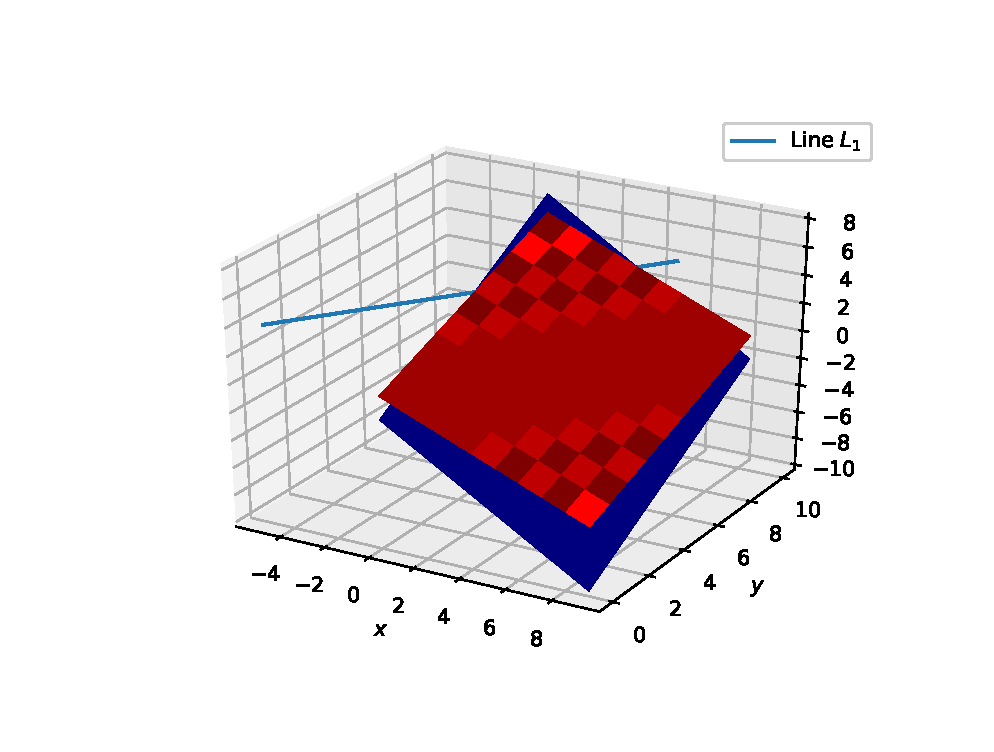
\includegraphics[width=\columnwidth]{./figs/1.1.eps}
\caption{}
\label{fig:1.1}
\end{figure}

\item $L_2$ is the intersection of the planes
\begin{align}
\myvec{1 & 2 & -1}\vec{x} &= 3
\\
\myvec{3 & -1 & 2}\vec{x} &= 1
\end{align}
Show that its equation is
%
\begin{align}
\vec{x} = \frac{1}{7}\myvec{ 5 \\ 8 \\ 0} + \lambda_2 \myvec{ -3 \\ 5 \\ 7}
\label{eq:l2}
\end{align}
\item Do $L_1$ and $L_2$ intersect? If so, find their point of intersection.
\\
\solution From \eqref{eq:l1},\eqref{eq:l2}, the point of intersection is given by
\begin{align}
\label{eq:l1l2pt}
\vec{x} = \frac{1}{7}\myvec{ 5 \\ 8 \\ 0} + \lambda_2 \myvec{ -3 \\ 5 \\ 7} &= \myvec{ 
-5 \\ 0 \\ 4} + \lambda_1 \myvec{ 1 \\ 1 \\ 0}
\\
\implies 
\myvec{1 &  3 \\ 1 & -5 \\ 0 & -7}\vec{\Lambda} &= \frac{1}{7}\myvec{40 \\ 8 \\ -28}
\end{align}
This matrix equation can be solved as
\begin{align}
\myvec{1 &  3 & \frac{40}{7}\\ 1 & -5 &\frac{8}{7}\\ 0 & -7 & -4} &\leftrightarrow \myvec{8 &  0 & 
\frac{224}{7}\\ 0 & 1 &\frac{4}{7}\\ 0 & 1 & \frac{4}{7} }
\\
\leftrightarrow \myvec{1 &  0 & 
4\\ 0 & 1 &\frac{4}{7} } &\implies \vec{\Lambda} = \myvec{4\\\frac{4}{7}}
\end{align}
%
Substituting $\lambda_1 = 4$ in \eqref{eq:l1l2pt}
\begin{align}
\vec{x} = \myvec{4 \\ 4 \\ 0} + \myvec{-5 \\ 0 \\ 4} = \myvec{-1\\ 4\\ 4}
\end{align}
\end{enumerate}
\section{Normal to a Plane}
\begin{enumerate}[label=\thesection.\arabic*
,ref=\thesection.\theenumi]
\item The cross product of $\vec{a},\vec{b}$ is defined as
\begin{equation}
\label{eq:cross}
\vec{a}\times \vec{b} = \myvec{0 & -a_3 & a_2 \\ a_3 & 0 & -a_1 \\ -a_2 & a_1 & 0}\myvec{b_1 \\ b_2 \\ b_3}
\end{equation}
From \eqref{eq:l1}, \eqref{eq:l2}, the direction vectors of $L_1$ and $L_2$ are
\begin{equation}
\myvec{1 \\ 1 \\ 0} \text{ and } \myvec{-3 \\ 5 \\ 7}
\end{equation}
respectively. Find the direction vector of the normal to the plane spanned by $L_1$ and $L_2$.
\\
\solution The desired vector is obtained as
\begin{align}
\myvec{1 \\ 1 \\ 0} \times \myvec{-3 \\ 5 \\ 7} = 
 \myvec{0 & 0 & 1 \\ 0 & 0 & -1 \\ -1 & 1 & 0}\myvec{-3 \\ 5 \\ 7}
= \myvec{7 \\ -7 \\ 8} = \vec{n}
\end{align}
\item Find the equation of the plane spanned by $L_1$ and $L_2$.
\\
\solution Let $\vec{x}_0$ be the intersection of $L_1$ and $L_2$.  Then the equation of the plane is
\begin{align}
\brak{\vec{x}-\vec{x}_0}^T\vec{n} &= 0
\\
\implies \vec{x}^T\vec{n} &= \vec{x}_0^T\vec{n}
\\
\implies \vec{x}^T\myvec{7 \\ -7 \\ 8} &= \myvec{-1 & 4 & 4}\myvec{7 \\ -7 \\ 8} =  -3
\end{align}
\item
Find the distance of the origin from the plane containing the lines $L_1$ and $L_2$.
\\
\solution The distance from the origin to the plane is given by
\begin{equation}
\frac{\abs{\vec{x}_0^T\vec{n}}}{\norm{n}} = \frac{1}{3\sqrt{2}}
\end{equation}
\end{enumerate}
\section{Projection on a Plane}
\begin{enumerate}[label=\thesection.\arabic*
,ref=\thesection.\theenumi]
%
\item Find the equation of the line $L$ joining the points 
\begin{align}
\vec{A}=\myvec{5 & -1 &4}^T
\\
\vec{B}=\myvec{4 & -1 & 3}^T
\end{align}
\solution The desired equation is
\begin{align}
\vec{x} &= \vec{B} + \lambda\brak{\vec{A}-\vec{B}}
\\
&= \myvec{4 \\ -1 \\ 3} + \lambda \myvec{1 \\ 0 \\ 1}
\label{eq:Lproj}
\end{align}
\item Find the intersection of $L$ and the plane $P$ given by
\begin{equation}
\myvec{1 & 1 & 1}\vec{x} = 7
\label{eq:Pproj}
\end{equation}
\\
\solution From \eqref{eq:Lproj} and \eqref{eq:Pproj},
\begin{align}
 \myvec{1 & 1 & 1}\myvec{4 \\ -1 \\ 3} + \lambda \myvec{1 & 1 & 1}
\myvec{1 \\ 0 \\ 1} &= 7
\\
\implies 6 + 2\lambda &= 7
\\
\implies \lambda &= \frac{1}{2}
\end{align}
%
Substituting in \eqref{eq:Lproj},
\begin{equation}
\vec{x} = \frac{1}{2}\myvec{9 & -1 & 7}
\end{equation}
\item Find $\vec{C} \in P$  such that $AC \perp P$.  
\\
\solution From \eqref{eq:Pproj}, the direction vector of $AC$ is $\myvec{1 & 1 & 1}^T$.  Hence, the equation of 
$AC$ is
\begin{equation}
\vec{x} = \myvec{5 \\ -1 \\ 4} + \lambda_1  \myvec{1 \\ 1 \\ 1}
\end{equation}
Substituting in \eqref{eq:Pproj}
\begin{align}
 \myvec{1 & 1 & 1}\myvec{5 \\ -1 \\ 4} + \lambda \myvec{1 & 1 & 1}
\myvec{1 \\ 1 \\ 1} &= 7
\\
\implies 8 + 3\lambda_1 &= 7
\\
\implies \lambda_1 &= -\frac{1}{3}
\end{align}
Thus,
\begin{align}
\vec{C} = \frac{1}{3}\myvec{14 \\ -4 \\ 11}
\end{align}
\item Show that if $BD \perp P$  such that $\vec{D} \in P$,
\begin{equation}
\vec{D} = \frac{1}{3}\myvec{13 \\ -2 \\ 10}
\end{equation}
%
\item Find the projection of $AB$ on the plane $P$.
\\
\solution The projection is given by
\begin{align}
CD = \norm{\vec{C}-\vec{D}} = \sqrt{\frac{2}{3}}
%\label{eq:homog}
\end{align}
\end{enumerate}
\section{Coplanar vectors}
\begin{enumerate}[label=\thesection.\arabic*
,ref=\thesection.\theenumi]
\item If $\vec{u}, \vec{A}, \vec{B}$ are coplanar, show that
\begin{equation}
\vec{u}^T\brak{\vec{A}\times \vec{B}} = 0
\label{eq:coplanar}
\end{equation}
%
\item Find $\vec{A}\times \vec{B}$ given
\begin{align}
\vec{A}=\myvec{2 & 3 & -1}^T
\\
\vec{B}=\myvec{0 & 1 & 1}^T
\end{align}
\solution From \eqref{eq:cross},
\begin{align}
\vec{A}\times \vec{B} &= \myvec{0 & 1& 3 \\ -1 & 0 & -2 \\ -3 & 2 & 0}\myvec{0 \\ 1 \\ 1}
\\
&= \myvec{4 \\ -2 \\ 2}
\label{eq:last_axb}
\end{align}

\item Let $\vec{u}$ be coplanar with 
%
such that $\vec{u}\perp\vec{A}$and
\begin{equation}
\vec{u}^T\vec{B} = 24.
\label{eq:uB}
\end{equation}
Find $\norm{\vec{u}}^2$.
\\
\solution From \eqref{eq:last_axb} and the given information,
\begin{align}
\vec{u}^T\myvec{4 & -2 & 2} &=0
\\
\vec{u}^T\myvec{2 & 3 & -1} &=0
\\
\vec{u}^T\myvec{0 & 1 & 1} &=24
\\
\implies \myvec{4 & -2 & 2
\\
2 & 3 & -1
\\
0 & 1 & 1
}\vec{u}
&= \myvec{0 \\ 0 \\ 24}
\\
\implies 
\vec{u} &= 4 \myvec{-1 \\ 2 \\ 4}
\\
\implies \norm{\vec{u}}^2 &= 336
\end{align}
\end{enumerate}
\section{Least Squares}
\begin{enumerate}[label=\thesection.\arabic*
,ref=\thesection.\theenumi]
\item Find the equation of the plane $P$
containing the vectors 
%
\begin{align}
\label{eq:least_vecs}
\vec{x}_1 = \myvec{1 \\ 1 \\ 1}
,
\vec{x}_2 = \myvec{0 \\ 1 \\ 2}
\end{align}
%
\item Show that the vector 
\begin{align}
\vec{y} = \myvec{6 \\ 0 \\ 0}
\end{align}
lies outside $P$.
\item Find the point $\vec{w} \in P$ closest to $\vec{y}$.
\item Show that
\begin{align}
\norm{\vec{y}-\vec{X}\vec{w}}^2 &= \norm{\vec{y}}^2 - \vec{w}^T\vec{X}^T\vec{y} 
\\
& \quad - \vec{y}^TA\vec{w}+\vec{w}^T\vec{X}^T\vec{X}\vec{w}
\end{align}
%
\item Assuming $2\times 2$ matrices and $2 \times 1$ vectors, show that
\begin{align}
\frac{\partial}{\partial\vec{w}}\vec{w}^T\vec{X}^T\vec{y} = \frac{\partial}{\partial\vec{w}}\vec{y}^T\vec{X}\vec{w} = 
\vec{y}^T\vec{X}
\end{align}
\item Show that
\begin{align}
\frac{\partial}{\partial\vec{w}}\vec{w}^T\vec{X}^T\vec{X}\vec{w} = 2\vec{w}^T\brak{\vec{X}^T\vec{X}}
\end{align}
\item Show that 
\begin{align}
\hat{\vec{w}} &= \min_{\vec{w}}\norm{\vec{y}-\vec{X}\vec{w}}^2
\\
 &= \brak{\vec{X}^T\vec{X}}^{-1}\vec{X}^T \vec{y}
\label{eq:least_sol}
\end{align}
\item Let 
\begin{align}
\vec{X} = \myvec{\vec{x}_1 & \vec{x}_2}.
\end{align}
from \eqref{eq:least_vecs}.
Verify \eqref{eq:least_sol}.
\end{enumerate}


\end{document}
